\chapter{مدل پیشنهادی}
\pagebreak
\section{مقدمه}
در فصل گذشته، روش‌های مطرح درک زبان طبیعی  معرفی شده و به بررسی هرکدام از روش‌ها پرداخته شد. از میان این روش‌ها، مدل \lr{Aligned CNN-BLSTM} \cite{Wang:18} به عنوان نقطه‌ی شروع این پایان نامه انتخاب شد. علت این امر، عملکرد مناسب این مدل در وظیفه‌ی پر کردن جای خالی، با وجود عدم استفاده از مدل‌های زبانی بود. به نظر می‌رسید مدل مذکور، با ایجاد تغییرات و استفاده از معماری‌های امروزی، بتواند عملکرد بهتری از خود نشان دهد. از طرف دیگر، \cite{Wang:18} در معماری خود از شیوه‌ی تراز کردن رمزگشا برای تولید تگ استفاده می‌کرد. شیوه‌ی تراز کردن \lr{LSTM} با رمزگشای ترنسفورمر سازگار نیست؛ از این رو جای خالی یک رمزگشای ترنسفورمر تراز شده نیز حس می‌شد. به همین دلیل، در این پایان‌نامه، مدل \lr{CTran}\LTRfootnote{\textbf{C}NN-\textbf{Tran}sformer} با تکیه بر شبکه‌ی کانولوشنی و ترنسفورمرها طراحی شد. در ادامه، ابتدا ساختار کلی معماری پیشنهادی را نمایش داده و سپس به تفصیل، اجزای سازنده‌ی آن توصیف می‌شود.

\section{طرح مدل}
معماری \lr{CTran} از یک رمزنگار مشترک، یک رمزگشای تشخیص هدف و یک رمزگشای پر کردن جای خالی تشکیل می‌شود. ابتدا جمله‌ی کاربر به عنوان ورودی، وارد رمزنگار شده و تعبیه‌ی میانی تولید می‌شود. این تعبیه‌ی میانی، به صورت همزمان وارد دو رمزگشا می‌شود. وظیفه‌ی رمزگشا در معماری، تولید خروجی‌های مدل است. هر رمزگشا، معماری منحصر به فردی دارد که برای وظیفه‌ی مورد نظرش طراحی گردیده است. برای اصلاح وزن‌های شبکه و آموزش مدل،خروجی‌های تولید شده با خروجی‌های مورد انتظار مقایسه شده و خطا محاسبه می‌شود. در مرحله‌ی بعد، وزن‌های هر رمزگشا به صورت جداگانه اصلاح می‌شود؛ اما از آن جا که رمزنگار بین دو وظیفه مشترک است، خطاهای هر دو وظیفه روی وزن‌های آن اثر می‌گذارند. در این بخش، ابتدا به معماری رمزنگار، سپس معماری رمزگشای تشخیص هدف و در پایان به معماری رمزگشای پر کردن جای خالی پرداخته می‌شود.
\begin{figure}[!htb]
	\centering
	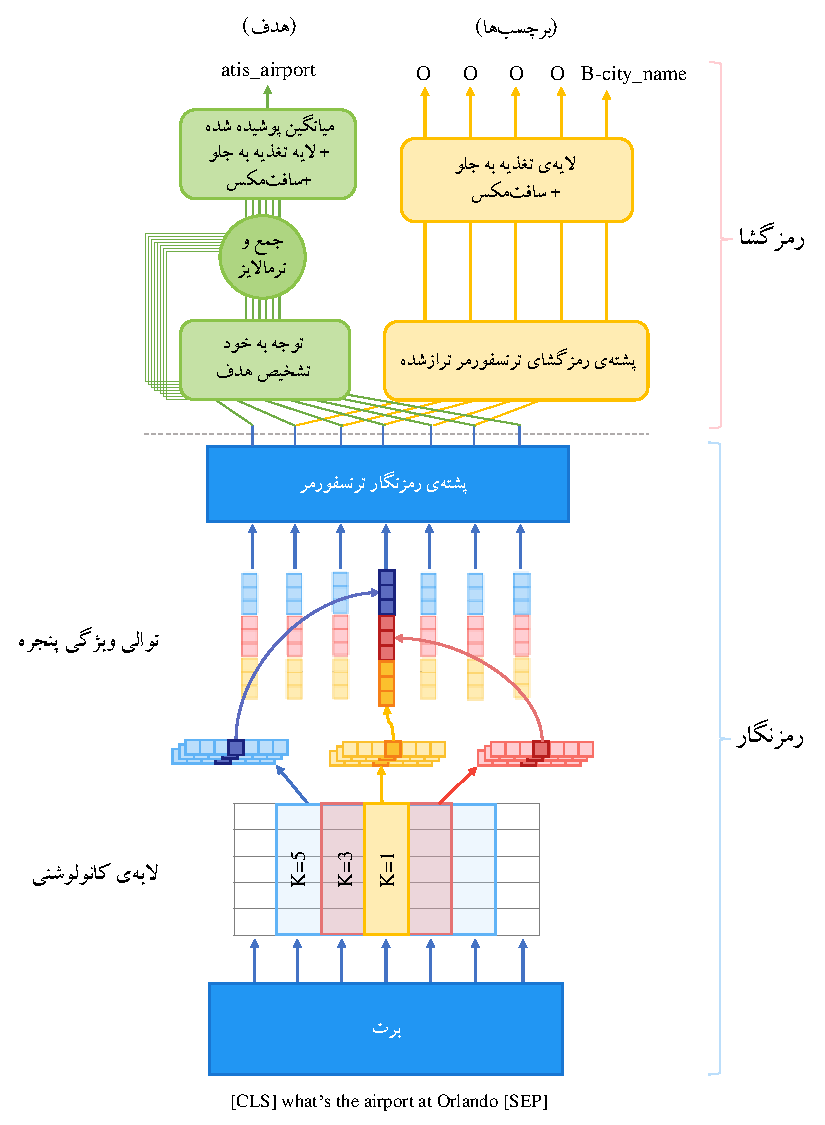
\includegraphics[scale=1]{Figures/modelarchitecture.pdf}
	\caption[معماری مدل پیشنهادی \lr{CTran}]{معماری مدل پیشنهادی \lr{CTran}. دو نشانه‌ی اضافه‌شده $[CLS]$ و $[SEP]$ از نشانه‌های ساختاری برت هستند. در زمان ورود تعبیه‌ی ایجاد شده به رمزگشای پر کردن جای خالی، تعبیه‌های متناظر با این دو نشانه، دور ریخته می‌شوند.}
	\label{Fig:architecture}
\end{figure}
\section{رمزنگار}
همانطور که گفته شد، \lr{CTran} از رمزنگار مشترک بهره می‌برد. رمزنگار شامل یک مدل زبانی پیش‌آموز شده، شبکه‌ی عصبی کانولوشنی، ساختار توالی ویژگی پنجره و پشته‌ی رمزنگار ترنسفورمر می‌شود. مطابق شکل \ref{Fig:architecture} در گام نخست، نشانه‌ها وارد مدل زبانی می‌شود تا تعبیه‌ای آگاه از پیش زمینه به دست آید. این تعبیه، به عنوان نقطه‌ی شروعی برای رمزنگار است. در گام بعد، این تعبیه‌ها وارد لایه‌ی کانولوشنی با اندازه هسته‌های مختلف می‌شود. استفاده از عملیات \lr{Max-Pooling} بعد از کانولوشن رایج است، اما با هدف حفظ توالی واژه‌ها، از ساختاری به نام توالی ویژگی پنجره استفاده شده است. در این ساختار، تمام بردارهای تولید شده برای یک واژه، ترانهاده شده و به یکدیگر الحاق می‌شوند. آخرین بخش رمزنگار، پشته‌ی رمزنگار ترنسفورمر است، که برای ایجاد تعبیه‌ی جدیدی که حاصل توالی ویژگی پنجره است، استفاده شده است. در ادامه، اجزاء سازنده‌ی رمزنگار تشریح می‌شوند.
\subsection{مدل زبانی پیش‌آموز شده}
اثبات شده که مدل‌های زبانی پیش‌آموز شده مانند برت و المو، برای بهبود عملکرد وظیفه‌های پردازش زبان طبیعی مفید هستند \cite{ethayarajh-2019-contextual}. در این پژوهش، هر دو مدل زبانی یاد شده در معماری پیشنهادی استفاده شده و نتایج آن‌ها مقایسه شدند.
ورودی برت جمعی تعبیه‌ی نشانه‌های \lr{WordPiece} \cite{wordpiece}، تعبیه‌ی موقعیتی و تعبیه‌ی بخش\LTRfootnote{Segment Embedding} می‌باشد. تعبیه‌ی بخش در مورد استفاده‌ی تک جمله‌ای معنا ندارد، چرا که تنها یک جمله وارد برت می‌شود. برای نشانه‌های ورودی $X=\left [x_{1},x_{2},x_{3},...,x_{L}\right ]$،  برت یک تعبیه‌ی آگاه به زمینه $H=\left [h_{1},h_{2},h_{3},...,h_{L}\right ]$ برای مدل فراهم می‌کند. توجه داشته باشید که نشانه ساز\LTRfootnote{Tokenizer} \lr{WordPiece} ممکن است واژه‌ها را به چند نشانه بشکند. این امر رابطه‌ی یک به یک واژه‌ی ورودی با برچسب را برهم میزند. همچنین، برچسب زدن نشانه‌های شکسته شده بیهوده است؛ چراکه همه‌ی آن‌ها به یک واژه تعلق داشته و برچسب یکسانی دارند. علاوه بر این، \lr{WordPiece} واژه‌های دارای علائم را نیز به چند نشانه می‌شکند. در روش پیشنهادی، این مشکل با حذف علائم درون واژه‌ها برطرف گردید. برای جلوگیری از حذف واژه‌هایی که فقط دارای علائم بوده و فاقد عدد و الفبا هستند، استثنا ایجاد گردید و علائم درون این واژه‌ها حذف نشدند. همچنین، همانطور که در بخش دو گفته شد، ورودی برت دارای نشانه‌های خاص است. این نشانه‌ها برای وظیفه‌ی پر کردن جای خالی در نظر گرفته نمی‌شوند.
	\\
برخلاف برت، نشانه ساز زبانی المو واژه‌ها را نمی‌شکند. از این رو ترتیب ورودی و خروجی یکسان است. در معماری پیشنهادی، از تعبیه‌های لایه‌ی آخر المو که حاوی تعبیه معنایی واژه‌ها است بهره برده شد.
\subsection{شبکه‌ی کانولوشنی}
در \cite{zhou:15clstm,Wang:18}، شبکه‌ی عصبی کانولوشنی برای پوشش کاستی‌های \lr{LSTM} استفاده شد. از آنجا که ترنسفورمر کاستی‌های یاد شده را برطرف کرده است، ممکن است استفاده از شبکه‌ی کانولوشنی بیهوده به نظر برسد. اما از طرفی، اثر استفاده از شبکه‌ی کانولوشنی در کنار ترنسفورمر برای وظیفه‌ی درک زبان طبیعی بررسی نشده است. در این پژوهش، از شبکه‌ی کانولوشنی، برای استخراج اطلاعات معنایی و همچنین ادغام آن‌ها در پنجره‌های مشخص استفاده شده است. این ویژگی از آن سو مورد توجه این پژوهش قرار گرفت، که ترنسفورمر، ذاتاً تفاوتی میان واژه‌های نزدیک به واژه‌ی اصلی و واژه‌های دورتر قائل نیست. این در حالی است که فرض اولیه‌ی مدل‌هایی مانند \lr{n-gram} \cite{ngram}، \lr{GloVe} و \lr{Word2Vec}، بر نقش کلیدی واژه‌های مجاور است. به همین علت، در معماری پیشنهادی، از چند لایه‌ی کانولوشنی، با اندازه هسته و مقادیر اولیه‌ی متفاوت استفاده شده، تا تعبیه‌ی واژه‌های همسایه با واژه‌ی مورد نظر آمیخته شود. این امر به منظور تاکید اثرگذاری واژه‌های همسایه بر معنای واژه‌ی فعلی است؛ امری که در \lr{LSTM} برای پوشش نقش دروازه‌ی ورودی صورت می‌گرفت.\\
اگر $d_{lm}$ نمایانگر بُعد تعبیه و جمله ورودی حاوی $L$ نشانه باشد، تعبیه‌ی جمله‌ی ورودی به صورت $h\in\mathbb{R}^{L\times d_{lm}}$ تعریف می‌شود و بردار تعبیه برای $i$-امین نشانه با $h_{i}\in \mathbb{R}^{d_{lm}}$ نشان داده می‌شود. اجازه دهید $k$ اندازه‌ی هسته باشد و $f\in\mathbb{R}^{k\times d_{lm}}$ یک هسته را نشان دهد. با این فرضیات، برای هر موقعیت $i$ در جمله، یک پنجره
 $w_{i}\in\mathbb{R}^{k\times d_{lm}}$
  وجود دارد که حاوی $k$ بردار نشانه بوده و به صورت $w_{i}=\left[h_{i},h_{i+1},h_{i+2}،\cdot،h_{i+k-1}\right]$ تعریف می‌شود. در صورتی که 
$\odot$
 ضرب عنصری، $b\in\mathbb{R}$ پارامتر بایاس و $A$ یک تابع فعال ساز باشد، عملیات کانولوشن $c_{i}$ برای هر پنجره $w_{i}$ توسط معادله‌ی \ref{Eq:Cnnoperation} محاسبه می‌شود. مدنظر داشته باشید که بعد از ضرب عنصری، تمام مقادیر ماتریس با یکدیگر جمع می‌شوند تا یک عدد به دست آید.
 \begin{equation}
 	c_{i}=A\left(w_{i}\odot f+b\right)
 	\label{Eq:Cnnoperation} 
 \end{equation}
این عملیات به ازاء $0<i<k$، یعنی تمام موقعیت‌های درون جمله انجام می شود. بر همین اساس، خروجی کانولوشن $f$ بر روی $x$ با $C=\left[c_{1},c_{2},c_{3},...,c_{i},...,c_{L}\right]$ نمایش داده می‌شود. لازم به ذکر است که در \lr{CTran} از پد صفر استفاده گردید؛ به همین دلیل اندازه‌ی ورودی و خروجی لایه‌ی کانولوشنی همواره برابر است. پد صفر برای حفظ برابر طول جمله‌ی خروجی با ورودی استفاده شد؛ چرا که در گام بعد، این بردارها با یکدیگر الحاق می‌شوند. از این رو، برابر بودن اندازه‌ی ورودی و خروجی اهمیت بالایی دارد.
\subsection{توالی ویژگی پنجره}
استفاده از عملیات \lr{Pooling} بعد از لایه‌ی کانولوشنی مرسوم است، اما نمونه بَرداری ناپیوسته\LTRfootnote{Discontinuous Sampling} باعث از دست رفتن برخی از اطلاعات می‌شود، و در نتیجه، این عملیات‌ها باعث از بین رفتن اطلاعات ترتیبی، در توالی داده‌ها می‌شود \cite{Wang:18}. در این پژوهش، به منظور حفظ ترتیب اصلی نشانه‌ها، از توالی ویژگی پنجره استفاده شد. در این ساختار، تعبیه‌ی نشانه‌ها با اندازه‌ی هسته‌ی مختلف و تعداد کانال خروجی مختلف، به یکدیگر الحاق می‌شوند تا یک بردار تعبیه برای آن نشانه تشکیل دهند.\\
فرض کنید $d_{conv}$ تعداد کل هسته‌ها، با اندازه‌ی هسته و مقادیر اولیه‌ی متفاوت برای هسته و $j$ بیانگر موقعیت $j$-امین فیلتر باشد. با در نظر گرفتن $\oplus$ به عنوان عملیات الحاق، $r_{i}\in\mathbb{R}^{d_{conv}}$ تعریف شده در معادله \ref{cnnfinal}، نمایش نهائی واژه‌ی $i$-ام را تعریف می‌کند و $C_{i}^{j}$ نشان دهنده $i$-امین عنصر فیلتر $j$-ام است.
\begin{equation}
	\label{cnnfinal}
	r_{i}=C_{i}^{1} \oplus C_{i}^{2} \oplus C_{i}^{3} \oplus ... \oplus C_{i}^{j} \oplus ... \oplus C_{i}^{d_{conv}}
\end{equation}
بنابراین $r_{i}$ تمام مقادیر کانولوشن متعلق به موقعیت $i$ را برای همه هسته‌ها به هم الحاق می‌کند.
این عملیات برای همه موقعیت‌ها انجام می‌شود تا زمانی که این نمایش برای همه واژه‌های ورودی تولید شود. خروجی ساختار توالی ویژگی پنجره، به شکل $R=\{r_{1},r_{2},r_{3},\cdots,r_{L}\}$ می‌باشد. در مرحله‌ی آخر، خروجی این ساختار به پشته‌ی رمزنگار ترنسفورمر تغذیه می‌شود تا نمایش نهائی تولید گردد.
\subsection{پشته‌ی رمزنگار ترنسفورمر}
امکان دسترسی مستقیم به تمام موقعیت‌های درون جمله، به رمزنگار ترنسفورمر کمک می‌کند تا بر از دست دادن اطلاعات غلبه کند. برتری آشکار ترنسفورمر باعث شد که از این شبکه، به جای  \lr{LSTM} استفاده شود.
پشته‌ی رمزگشای ترنسفورمر، همانطور که در شکل \ref{Fig:bert} نشان داده شد، از چندین لایه تشکیل شده است که در آن، خروجی هر لایه به عنوان ورودی لایه بعدی استفاده می‌شود. با توجه به ساختار رمزنگار ترنسفورمر، ابعاد خروجی آن برابر با ورودی است؛ یعنی خروجی این لایه برابر با $H\in\mathbb{R}^{L\times d_{conv}}$ می‌باشد.

\section{رمزگشا}
ماتریس ایجاد شده در رمزنگار $H$، که در این پایان‌نامه حافظه نامیده شده، به صورت همزمان به دو رمزگشا تغذیه می‌شود. این ماتریس به عنوان نقطه‌ی آغاز شبکه‌های رمزگشا است. هرکدام از این دو رمزگشا، تغییرات متناسب با ساختار احتمالات خروجی را، بر روی ماتریس ایجاد می‌کنند. در ادامه، شبکه‌های پیشنهادی برای رمزگشای تشخیص هدف و رمزگشای پر کردن جای خالی معرفی می‌شوند.
\subsection{رمزگشای تشخیص هدف}
همانطور که در شکل \ref{Fig:architecture} ترسیم شده، رمزگشای تشخیص هدف از یک لایه‌ی توجه به خود با اتصال باقی‌مانده و لایه‌ی نرمال سازی تشکیل شده است. معادله‌ی \ref{Eq:intent_attention} بیانگر عملیات یاد شده است. 
\begin{equation}
	D_{intent} = H + LayerNorm(  MultiHead(H)  )
	\label{Eq:intent_attention}
\end{equation}
 در ادامه، یک لایه‌ی تغذیه به جلو و سافت‌مکس برای محاسبه‌ی احتمالات خروجی مورد بهره‌وری قرار گرفته است. بر این اساس، ابتدا میانگین تعبیه‌ی نشانه‌های درون جمله محاسبه می‌شود. در محاسبه‌ی این میانگین، تعبیه‌ی نشانه‌هایی که برای پد کردن جمله اضافه شده‌اند نادیده گرفته می‌شود؛ بدین جهت، این میانگین، پوشیده نامیده شده است. بعد از اعمال میانگین پوشیده، طول جمله $L$ در خروجی مرحله قبل $D_{intent}\in\mathbb{R}^{L\times V}$، فرو می‌ریزد و این ماتریس تبدیل به یک بردار $D_{intent}^{\prime}\in\mathbb{R}^{1\times V}$ می‌شود. با در نظر گرفتن محصول نقطه‌ای با علامت $\cdot$، تعداد اهداف یکتای مجموعه داده با $I$، وزن‌ها $w\in\mathbb{R}^{V\times I}$
و بایاس $b\in\mathbb{R}^{1\times I}$ که هردو مورد اخیر قابل آموزش هستند، احتمالات خروجی $P_{intent}\in\mathbb{I}^{1\times I}$\RTLfootnote{علامت $I$ بیانگر فضای واحد (\lr{Unit Interval}) می‌باشد.} برای وظیفه‌ی تشخیص هدف، با معادله‌ی \ref{Eq:decoder_id} محاسبه می‌شود.
\begin{equation}
	P_{intent} = softmax( w\cdot D_{intent}^{\prime} + b )
	\label{Eq:decoder_id}
\end{equation}

\subsection{رمزگشای پر کردن جای خالی}
رمزگشای پیشنهادی برای پر کردن جای خالی از دو قسمت تشکیل شده است؛ یک رمزگشای ترنسفورمر تراز شده و یک لایه‌ی تغذیه به جلو برای کاهش ابعاد خروجی به تعداد برچسب‌های یکتای مجموعه داده.\\
 از آنجایی که واژه‌های ورودی با برچسب‌های هدف رابطه‌ی یک به یک دارند، بهتر است رمزگشا تراز شده باشد. تراز بودن به این معناست که مدل از نشانه، یا موقعیتی که درحال حاضر برچسب آن را تولید می‌کند، آگاه باشد. این آگاهی باید صریح باشد؛ یعنی مدل مستقیماً به بردار تعبیه‌ی آن نشانه دسترسی داشته باشد. این آگاهی به معنای دسترسی مستقیم به تعبیه‌ی آن نشانه است. تا به حال، روشی برای تراز کردن رمزگشای ترنسفورمر پیشنهاد نشده است؛ از این رو، در این پژوهش، رمزگشای ترنسفورمر تراز شده ابداع می‌شود. ترازی مورد نظر، در بخش توجه متقابل صورت می‌گیرد؛ جایی که کلید و مقدار از حافظه تولید می‌شود. برای پوشاندن حافظه، یک ماسک با اندازه‌ی $(S,T)$ نیاز است، که $S$ نشان دهنده‌ی طول ترتیب مبدا و $T$ نشان دهنده‌ی طول ترتیب مقصد است. از آنجا که طول مبدا و مقصد در وظیفه‌ی برچسب زنی ترتیب یکسان است، ماسک مورد استفاده‌ی به شکل $(S,S)$ تعریف می‌شود. در این پژوهش، رمزنگار ترنسفورمر با استفاده از ماتریس قطری\LTRfootnote{Diagonal Matrix} $M_{diagonal}\in\mathbb{R}^{S\times S}$ برای ماسک حافظه، تراز شد. ماتریس قطری، نوعی ماتریس است که تمام موقعیت‌ها بجز $s=t$ صفر هستند. در این تعریف $s$ بیانگر موقعیت ردیف و $t$ موقعیت ستون ماتریس است. در واقع، تمام عناصر صفر این ماتریس تبدیل به $-inf$ شده و قطر آن تبدیل به صفر می‌شود. این کار به قصد آن صورت می‌گیرد که پس از جمع کردن آن با ماتریس وزن‌های توجه، باعث نامعتبر شدن تمام موقعیت ها، بجز موقعیت متناظر با برچسب درحال تولید شود.  از این رو، مکانیزم توجه متقابل و متعاقباً رمزگشای ترنسفورمر، تنها بردار تعبیه‌ی موقعیتی که در جمله‌ی مبدا، مربوط به برچسب درحال تولید است را در نظر می‌گیرد.\\
 مانند رمزگشای ترنسفورمر، نسخه‌ی تراز شده‌ی آن نیز ازنظر کاربرد به سه بخش تقسیم می‌شود.
 با تعریف تبدیل خطی پرسش $Q\in\mathbb{R}^{d_{conv}}$، کلید $K\in\mathbb{R}^{d_{conv}}$ و مقدار $V\in\mathbb{R}^{d_{conv}}$ از تعبیه‌ی برچسب‌های هدف $E_{target}\in\mathbb{R}^{L\times d_{conv}}$، نخستین بخش رمزگشای ترنسفورمر تراز شده، مطابق معادله‌ی \ref{Eq:aligned_dec1} مکانیزم توجه به خود، بر روی تعبیه‌ی برچسب‌ها است که برای درک روابط میان برچسب‌های پیشین استفاده شده است.
 \begin{equation}
 	D_{slots} = E_{target} + LayerNorm(MultiHead_{masked}(Q,K,V,M_{upper}))
 	\label{Eq:aligned_dec1}
 \end{equation}
علت برابری تعداد بُعد تعبیه‌ی برچسب‌های هدف با بعد حافظه، سازگاری این دو برای انجام عملیات توجه متقابل است.\\
بخش دوم رمزگشای ترنسفورمر، توجه متقابل است. ترازی در این بخش تعریف شد تا از توجه رمزگشا به موقعیت‌هایی که متناظر با برچسب درحال پردازش نیستند، جلوگیری کند. با در نظر گرفتن تبدیل خطی پرسش $Q\in\mathbb{R}^{d_{conv}}$ از $C$، کلید $K\in\mathbb{R}^{d_{conv}}$ و مقدار $V\in\mathbb{R}^{d_{conv}}$ از حافظه $H$، خروجی لایه‌ی توجه متقابل تراز شده پیشنهادی، با استفاده از معادله‌ی \ref{Eq:aligned_dec2} به دست می‌آید.
  \begin{equation}
 	D_{slots} \prime = D_{slots} + LayerNorm(MultiHead_{masked}(Q,K,V,M_{diagonal}))
 	\label{Eq:aligned_dec2}
 \end{equation}
 بخش آخر رمزگشای ترنسفورمر تراز شده، یک لایه‌ی تغذیه به جلو است.
 \begin{equation}
 	D_{slots} \prime\prime = D_{slots}\prime + LayerNorm(FeedForward(D_{slots}\prime))
 	\label{Eq:aligned_dec3}
 \end{equation}
در پایان، برای به دست آوردن احتمال برچسب‌های خروجی $P_{slots}\in\mathbb{I}^{L\times T}$، با استفاده از معادله‌ی \ref{Eq:aligned_dec4}، به تمام برچسب‌های موجود در واژه‌نامه‌ی هدف $T$، احتمالی بین ۰ و ۱ اختصاص داده می‌شود.
\begin{equation}
	P_{Slots} = Softmax(LinearLayer(D_{slots}\prime\prime))
	\label{Eq:aligned_dec4}
\end{equation}


\section{تفسیر خروجی} %چجوری توکن خروجی رو برمیداری
همانطور که در بخش رمزگشا گفته شد، مدل یک خروجی احتمالاتی تولید می‌کند؛ به این معنا که به ازاء تمام برچسب‌های یکتا و همچنین به ازاء تمام هدف‌های یکتای موجود در مجموعه داده، عددی بین ۰ تا ۱ تولید می‌کند. اما برای استفاده از خروجی شبکه، باید سیاستی برای انتخاب خروجی شبکه از میان احتمالات وجود داشته باشد. در این پایان نامه، سیاست حریصانه  برای انتخاب برچسب و هدف استفاده شده است. سیاست حریصانه در انتخاب هدف، به معنای انتخاب کلاسی است که بیشترین احتمال وقوع را دارد. برای بهره‌وری از این سیاست در وظیفه‌ی پر کردن جای خالی، در هر موقعیت از جمله، برچسبی که بیشترین احتمال وقوع را دارد انتخاب می‌شود.